\immediate\write18{bibtex \jobname}
\documentclass{amsart}
\usepackage{amsmath, amsthm, amssymb}
\usepackage[colorlinks=true,linkcolor=blue,urlcolor=blue]{hyperref}
\usepackage[capitalize,noabbrev]{cleveref}
\usepackage{tikz-cd}
%\usepackage{newtxtext,newtxmath}
\usepackage[numbers,sort,compress]{natbib}
\usepackage{graphicx}

%To-do
\usepackage[marginpar]{todo}
\makeatletter
\renewcommand{\@tododisplay}[1]{%
%\marginpar{#1}%
\textsuperscript{#1}%
}
%
\renewcommand\@displaytodo[2][\todomark]{%
\@tododisplay{{\todoformat [#1~\ref{todolbl:\thetodo}]}}%
\footnotetext[\thetodo]{\todoformat #1:~#2}%
\global\@todotoks\expandafter{\the\@todotoks\todoitem{#1}{#2}}%
\@todotrue%
}%
\renewcommand\todomark{todo}
\makeatother

% theorems
\theoremstyle{plain}
\newtheorem{thm}{Theorem}[section]
\Crefname{thm}{Theorem}{Theorems}
\newtheorem{cor}[thm]{Corollary}
\newtheorem{lem}[thm]{Lemma}
\newtheorem{prop}[thm]{Proposition}
\Crefname{prop}{Proposition}{Propositions}
\newtheorem{claim}[thm]{Claim}
\newtheorem{conj}[thm]{Conjecture}
\Crefname{conj}{Conjecture}{Conjectures}
\theoremstyle{definition}
\newtheorem{defi}[thm]{Definition}
\newtheorem{ex}[thm]{Example}
\newtheorem{rem}[thm]{Remark}

% commands
\newcommand{\N}{\mathbb{N}}
\newcommand{\Z}{\mathbb{Z}}
\newcommand{\R}{\mathbb{R}}
\newcommand{\HS}{\mathrm{HS}}
\newcommand{\HT}{\mathrm{HT}}
\newcommand{\HLC}{\mathrm{HLC}}
\renewcommand{\H}{\mathbb{H}^d}
\newcommand{\dprime}{{\prime\prime}}
\DeclareMathOperator{\interior}{int}
\DeclareMathOperator{\im}{im}
\newcommand\CH{\check{H}}

% margins
\setlength{\textwidth}{\paperwidth}
\addtolength{\textwidth}{-1.6in}
\setlength{\textheight}{\paperheight}
\addtolength{\textheight}{-1.8in}
\calclayout

\newcommand{\anibal}[1]{\textcolor{blue}{[Anibal: #1]}}

\begin{document}

\title[Persistence in functional topology]{Persistence in functional topology: q-tameness, local-connectivity and a correction to a theorem of Morse}
\author{}
\date{\today}

\begin{abstract}
With applications to the study of minimal surfaces in mind, Marston Morse wrote a series of papers developing versions of his famous inequalities for a broad class of real-valued functions on metric spaces. His work is remarkable in so far as it likely represents the first use of something that can be called persistent homology in the mathematical literature. From the modern point of view, it is particularly interesting that he uses Vietoris homology in order to enforce semi-continuity of persistent homology and that he states two topological conditions that supposedly ensure q-tameness. However, he is partly incorrect: We present a filtration that satisfies one of his conditions but has non-q-tame persistent homology. We also conjecture that his other condition, for which he provides no proof, is correct and discuss possible proof strategies.
\end{abstract}

\maketitle

%!TEX root = ../func_top.tex

\section{Introduction}

The interplay between the critical set of a function and the topology of its domain is a cornerstone of modern mathematics.
Nowadays, when thinking about the pioneering work of Marston Morse, our first thought probably involves a differentiable function on a closed smooth manifold, but more general settings should also be considered.
Morse theory in the smooth context was masterfully presented in Milnor's famous book on the subject \cite{Milnor.1963}, where he also gave a new proof of Bott's periodicity by applying Morse theory to the energy functional of paths in a Riemannian manifold, which notably goes beyond the compact setting.
Another important example of the use of Morse's insights in an infinite-dimensional context is Floer's work on the Arnold conjecture and its many ramifications in symplectic topology, as surveyed for example in \cite{Salamon.1999}.
Morse himself worked in a very general setting, publishing in the 1930s a pair of papers \cite{Morse.1937, Morse.1940} and a monograph \cite{Morse.1938} in which he established the key results of Morse theory in the broad context defined by semi-continuous functionals on metric spaces.
He called the theory set forth in this body of work \emph{functional topology} and used it to study questions about minimal surfaces motivated by Douglas' solution to Plateau’s Problem \cite{Douglas.1931}.
In particular, Morse and Tompkins \cite{Morse.1939} used these techniques to prove a general \emph{Mountain Pass Theorem} --~an existence result for saddle points~-- applying to functions that are not necessarily continuous (\cref{thm:mountain_pass}).
From this, they deduce their \emph{Unstable Minimal Surface Theorem}, showing the existence of critical points of the Douglas functional that are not local minima (\cref{thm:unstable_minimial_surface}).
In the intervening years, this result has been reproven and generalized in several directions using various techniques, and the problem class is still an active area of research \cite{Struwe.1984,Jost.1990,Jost.1991,Montezuma.2020,Marques.2021}.

Morse's work on functional topology did not have a long lasting impact on minimal surface theory or the calculus of variations in general; possibly in part because, as expressed by Struwe:
\begin{displaycquote}[p.~82]{Struwe.1988}
	The technical complexity and the use of a sophisticated topological machinery [...] tend to make Morse--Tompkins' original paper unreadable and inaccessible for the non-specialist.
\end{displaycquote}
A similar assessment was given by Bott, who writes in \cite[p.~934]{Bott.1980} that the papers \cite{Morse.1937, Morse.1940} ``are not easy reading'' and constitute a ``tour de force'' by Morse.

The intricacies of Morse's development notwithstanding, many of his ideas have subsequently resurfaced and flourished in other domains.
In particular, in applied topology and symplectic geometry, several key insights of Morse have been independently rediscovered as part of the development of \emph{persistent homology}, a technique that provides robust and efficiently computable invariants of filtered spaces using the functorial properties of homology.
Its success in these fields has motivated a refined abstract theory of persistence that lies in the intersection of geometry, topology, and representation theory.

The homology of a filtered space is an example of what is referred to as a \emph{persistence module}, a functor to vector spaces from the real numbers considered as a poset category.
In many important cases, a persistence module $M$ admits an essentially unique decomposition into indecomposable direct summands, and the structure of this decomposition yields a complete invariant of $M$ known as its \emph{persistence diagram}.
The set of all persistence diagrams can be organized into a metric space.
This often allows to recast geometric questions about general filtered spaces in a combinatorial metric model, since the passage via the homology construction to this metric space is Lipschitz, a statement commonly known as the \emph{stability} of persistence diagrams.

The most remarkable connections between functional topology and persistence theory come from Morse's paper \cite{Morse.1940}, where he developed the theory of \emph{caps} and their \emph{spans}.
They capture much of the same information as the modern notion of persistence diagram, including concepts such as the persistence or birth and death of a homology class, although Morse's results still fall short of yielding global decompositions of persistence modules.
Morse used his theory of caps to study functionals on a metric space by analyzing the evolution of the topology of their sublevel sets.
A key tool to this end is a version of his eponymous inequalities for cap numbers, which expands their usual version in the compact and smooth setting.
In this work, using persistence diagrams, we generalize the definition of these cap numbers to persistence modules and prove the existence of Morse inequalities for a large class of them (\cref{t:inequalities}).
Our approach makes these inequalities accessible in new contexts beyond those originally covered by functional topology.

Given the importance of persistence diagrams, in particular for stating and proving Morse inequalities, our focus will then be on the study of topological properties ensuring their existence for a broad class of filtered spaces and homology constructions.
For general persistence modules, a well studied condition for the existence of persistence diagrams is \emph{q-tameness} \cite{Chazal.2016a,Chazal.2016b}, which simply states that all linear maps between different real values in the persistence module have finite rank.
This condition is satisfied by a large class of important constructions; for example, the Vietoris--Rips or \v Cech persistent homology of a totally bounded metric space is q-tame \cite{Chazal.2014}.
The motivating question can then be reformulated as asking for topological conditions on a filtered space that ensure its persistent homology to be q-tame.
We now present the answers provided in the present work.

The persistence module associated to a filtration depends on the homology construction used, which, even when agreeing on cellular spaces, need not coincide for general topological spaces.
We restrict attention to homotopy invariant functors to the category of graded vector spaces satisfying the Mayer--Vietoris property for either open or closed sets, the primary examples being singular homology and \v{C}ech homology, respectively.

The sublevel set filtration $f_{\leq t} = f^{-1}(-\infty, t]$ of a real valued function $f$ is called \emph{locally homologically small} or \emph{$\HLC$} for a given homology theory if for any $x \in X$, any neighborhood $V$ of $x$, and any pair of indices $s,t$ with $f(x) < s < t$, there is a neighborhood $U$ of $x$ with $U \subseteq V$ such that the inclusion $f_{\leq s} \cap U \hookrightarrow f_{\leq t} \cap V$ is \emph{homologically small}; that is to say, the induced map in homology has finite rank in every degree.
We say that a sublevel set filtration is \emph{compact} if all sublevel sets are compact Hausdorff spaces.
We can now state our main result (\cref{t:local connectedness implies q-tameness}):

\begin{thm*}
	If the sublevel set filtration of a function $f \colon X \to \R$ is compact and	$\HLC$, then its persistent homology is q-tame.
\end{thm*}

\noindent We also introduce a weaker local-connectivity condition that can be used instead of $\HLC$ in the statement above if the filtration is defined by a continuous functional (\cref{c:q-tameness for continuous functions}).

To illustrate the applicability of our results we return to the original setting of the Douglas functional that motivated the development of functional topology.
This functional satisfies the hypotheses of \cref{t:local connectedness implies q-tameness}, so its associated persistent \v{C}ech homology is indeed q-tame and admits a persistence diagram.
From this, one can easily deduce the existence of an unstable minimal surface.
As it turns out, the local connectivity conditions proposed by Morse \cite{Morse.1938,Morse.1939,Morse.1940} are not sufficient for this purpose, which we illustrate by a counterexample (\cref{c:counterexample}).


\subsection*{Summary}

The primary contribution of this work consists in a modern development of the homological aspects of Morse's functional topology from the perspective of persistence theory.
We adjust several key definitions and prove stronger statements -- including a generalized version of the Morse inequalities -- in order to allow for novel uses of persistence techniques in the calculus of variations.
We provide sufficient conditions for a lower semicontinuous function to have q-tame persistent sublevel set homology, and hence to admit a persistence diagram.
As an application of these results, we correct an inaccuracy in a result by Morse, which was employed in the proof of the Unstable Minimal Surface Theorem given by Morse and Tompkins.


\subsection*{Outline}

In \cref{s:persistence} we recall the foundations of persistence theory, considering the persistent homology of a sublevel set filtration as the key example.
We present a persistence-theoretic point of view on Morse inequalities in \cref{s:inequalities}.
It generalizes both their versions in the smooth and compact setting as well as the one used in functional topology.
The main result of the present work is presented in \cref{s:connectivity}, where we define two natural notions of local-connectivity for a sublevel set filtration and show under what circumstances they imply q-tameness of its associated persistence module.
We close in \cref{s:surfaces} with a historical overview of Morse--Tompkins' application of functional topology to minimal surface theory, and we explore its relation to our results.
\cref{s:vietoris} contains a brief discussion on the definitions of Vietoris and \v{C}ech homology and their equivalence for compact metric spaces.


\section{Preliminaries}

\begin{itemize}
	\item metric space
	\item upper semi-continuous function
	\item Persistence module
	\item q-tameness
	\item Barcode
	\item bottleneck
	\item stability
\end{itemize}

\begin{defi}
	Let $M$ be a metric space. For any $p \in M$ and $\epsilon \geq 0$ denote
	\begin{equation*}
	B_\epsilon(p) = \{q \in M\ |\ d(p,q) < \epsilon\}, \qquad
	\overline B_\epsilon(p) = \{q \in M\ |\ d(p,q) \leq \epsilon\}.
	\end{equation*}
\end{defi}

\begin{defi}
	Let $X$ be a space and $f \colon X \to \R$ a function. For any $t \in \R$, the \textit{$t$-sublevel set of $f$} is defined by 
	\begin{equation*}
	X_{\leq t} = f^{-1}((-\infty, t]).
	\end{equation*}
\end{defi}

\section{Local connectivity and q-tameness}

Let $\H$ be a fixed homology theory.

\begin{defi} \label{defi:local_connectedness}
	For $n \in \Z$ a continuous map is said to be \textit{$n$-homologically small} or \textit{trivial}, denoted $\HS_n$ and $\HT_n$ respectively, if the image of the map induced by $\H_n$ is finitely generated or 0, and we say it is \textit{homologically small} or \textit{trivial}, denoted respectively $\HS$ and $\HT$, if it is $\HS_n$ or $\HT_n$ for every~$n$.
\end{defi}

\begin{defi}
	A space $X$ is said to be \emph{homologically locally connected}, denoted $\HLC$, if for each $x \in X$ any neighborhood $V$ of $x$ contains a neighborhood $U$ of $x$ such that the inclusion $U \to V$ is $\HT$.
\end{defi}

Local connectivity assumptions have a long history of being used to ensure that different homology theories agree and to ensure that homology is finite dimensional, see \cite{MR0007094} for early examples.
For us, the following is relevant.
Recall that a space is said to be \textit{paracompact} if every open cover has a locally finite open refinement, i.e., every point has a neighborhood intersecting finitely many sets in the refinement.

\begin{prop}[{\cite{MR105677, MR1481706}}] \label{prop:cech_sing_hom_hlc}
	On the category of paracompact Hausdorff $\HLC$ spaces, \v{C}ech and singular homology with arbitrary coefficients coincide.
\end{prop}

For more results of this type, we refer to \cite{MR1481706}. There, the above proposition \cite[Corollary VI.12.6]{MR1481706} and many similar ones are proven using sheaf theoretic methods.
For example, Bredon also discusses cohomology local connectedness \cite[Section II.17]{MR1481706} and various other comparison results, e.g.\@ between singular and Borel-Moore homology \cite[Corollary V.12.15]{MR1481706} in the presence of homology local connectedness, as well as examples such as spaces that are sheaf cohomology locally connected but not homology locally connected \cite[Example II.17.12]{MR1481706}.

For sublevel filtrations we obtain the following persistence version of Proposition~\ref{prop:cech_sing_hom_hlc} obtained by applying it pointwise.

\begin{cor}\label{cor:cech_sing_persistent_iso}
	Let $(X, f)$ be a sublevel filtration. If each sublevel set is paracompact and $\HLC$, then its singular and \v{C}ech persistence modules coincide.
\end{cor}

We are interested in statements that bound the dimension of homology with field coefficients.
In the non-filtered context one has the following result.

\begin{prop} \label{prop:fin_dim_sing_hom}
	Let $X$ be a compact Hausdorff $\HLC$ space.
	Then the singular homology of $X$ with field coefficients is finite-dimensional in every degree.
\end{prop}

\begin{proof}
	By the universal coefficient theorem for homology, trivial singular homology with integer coefficients also implies trivial singular homology for any other coefficient group. In particular, this means that $X$ being $HLC^{\infty}$ also implies that $X$ is $HLC^{\infty}_{\mathbb{F}}$. By the universal coefficient theorem for cohomology, the singular cohomology with coefficients in $\mathbb{F}$ is naturally isomorphic to the dual space of the singular homology with coefficients in $\mathbb{F}$. This means that being $HLC^{\infty}_{\mathbb{F}}$ implies being locally connected with respect to singular cohomology in all degrees with coefficients in $\mathbb{F}$. Since we assume $X$ to be $HLC^{\infty}$, \cite[Theorem III.1.1]{MR1481706} now implies that $X$ is locally connected with respect to sheaf cohomology with coefficients in the locally constant sheaf with value $\mathbb{F}$. \cite[Corollary II.17.7]{MR1481706} implies that the sheaf cohomology of the whole space with coefficients in this sheaf is finite-dimensional, so again by \cite[Theorem III.1.1]{MR1481706} the same holds for singular cohomology with coefficients in $\mathbb{F}$. Applying the universal coefficient theorem once more proves the claim.
\end{proof}

Again, there is a persistent version for sublevel filtrations.

\begin{cor}
	Let $(X, f)$ be a sublevel filtration. If each sublevel set is compact and $\HLC$, then its singular persistence module is p.f.d. in every degree, in particular q-tame.
\end{cor}

Having each space in a sublevel filtration being $\HLC$ is in many cases too restrictive.
We would like a relative condition for sublevel filtrations to be sufficient to ensure the q-tameness of the associated persistence module.

\begin{defi} \label{defi:local_connectedness_filtrations}
	For a fix homology theory $\H$. A sublevel filtration $(X,f)$ is said to be $\HLC$ if for any $\epsilon > 0$, $x \in X$, and $V$ an open neighborhood of $x$, there is a $\delta \in (0, \epsilon)$ and a neighborhood $U$ of $x$ such that $U \subseteq V$ and
	\begin{equation*}
	X_{\leq f(x) + \delta + c} \cap U \to X_{f(x) + \epsilon + c} \cap V
	\end{equation*}
	is $\HT$ for every $c \geq 0$.
	We also consider a weaker version, referred to as \textit{weakly} $\HLC$, defined as above with $c = 0$.
\end{defi}

We remark that if $\H$ is singular homology, both conditions of $\HLC$ for a Morse filtration $(M,f)$ are respectively equivalent to Morse's definitions of locally $f$-connectedness when $M$ is a metric space.
Please consult the historical recount presented in Section~\ref{sec:historical}.

We will now show that the weak notion does not imply q-tameness in general.
To do so let us consider the \textit{$d$-dimensional Hawaiian earring}
\begin{equation*}
\HE = \bigcup_{n\in\mathbb{N}}\left\{(x_0,\dots,x_d)\in\R^{d+1} \ \middle | \ \left(x_0-\frac{1}{n}\right)^2+x_1^2+\dots+x_d^2=\left(\frac{1}{n}\right)^2\right\}.
\end{equation*}

\begin{figure}[t]
	\centering
	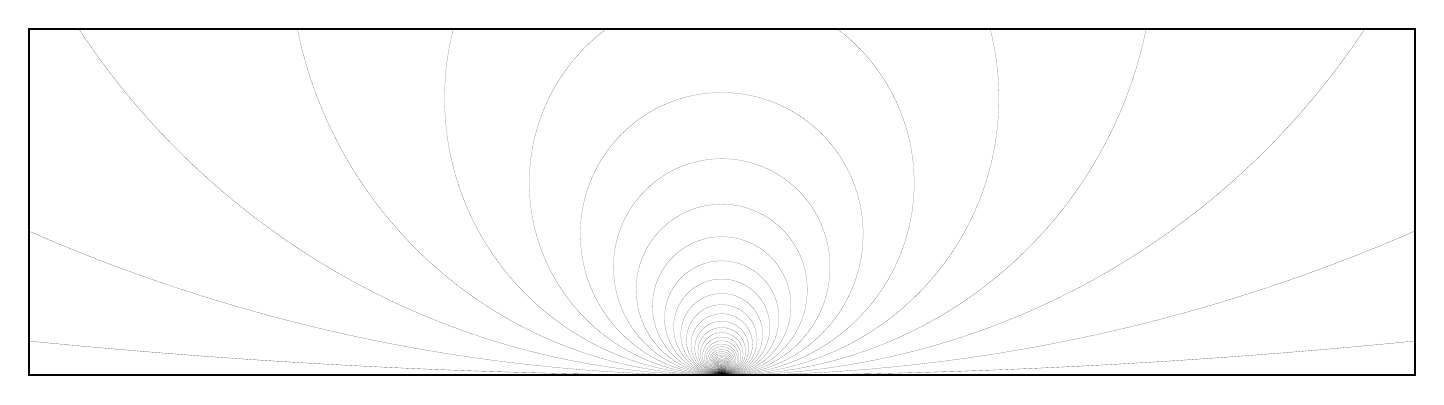
\begin{tikzpicture}[scale=88]
	\draw[thick] (-.1,0) rectangle (.1,.05);
	\clip (-.1,0) rectangle (.1,.05); % remove for all circles
	\foreach \i in {1,...,100}{
		\draw[line width=0.1/\i mm] (0, 1/\i^2) circle (1/\i^2);
	}
	\end{tikzpicture}
	\caption{A closeup of the Hawaiian hearing $\mathbb{H}^1$.}
	\label{fig:earrings}
\end{figure}

\begin{thm} \label{thm:counterexample}
	Let $\H$ be a homology theory such that its value on a point is finitely generated for every degree and on $\HE$ is not finitely generated for some degree. Then, the function $f \colon \HE \to \R$ whose value at the origin is $0$ and is $1$ everywhere else defines a $\HLC$ Morse filtration that is not q-tame.
\end{thm}

\begin{proof}
	The space $\HE$ is Hausdorff and locally compact since $R^{d+1}$ is.
	To verify that $(\HE,f)$ is a Morse filtration we notice that all level sets are either the empty set, the singleton containing the origin, or $\HE$ itself, all compact spaces.
	Let us now verify that $\HE$ is $\HLC$.
	Let $\epsilon > 0$ and $x \in \HE$.
	If $x$ is the origin, we choose $\delta$ between $0$ and the minimum of $\epsilon$ and $1$.
	Then $\HE_{\leq f(x) + \delta} = \HE_{\leq \delta} = \{x\}$, so the desired condition follows from the first assumption on the homology theory.
	For $x$ not the origin, there is a unique $d$-sphere that contains it.
	Clearly, we may choose $\delta > 0$ so small that $D_\delta(x) = \{y \in \R^{d+1} \mid \Vert x - y \Vert < \delta\} \cap \HE$ is contained in this sphere, so $D_\delta(x)$ is homotopy equivalent to a $x$ and the condition again follows trivially.
	What remains to be shown is that $\HE_{\leq \bullet}$ is not q-tame.
	Since $\HE_{\leq t}$ is constant with value $\HE$ for $t \geq 1$, the second assumption on the homology theory finishes the proof.
\end{proof}

The theories that we are most interested in do satisfy these conditions.

\begin{prop}
	The assumptions of Theorem~\ref{thm:counterexample} are satisfied by singular homology with any coefficients and \v{Cech} homology with field coefficients.
\end{prop}

\begin{proof}
	The case of singular homology is well know and can be found in \cite{Barratt.1962}.
	For \v{C}ech homology we use the fact that it commutes with inverse limits for compact Hausdorff spaces.
	Define 
	\begin{align*}
	\HE_k &= \left\{(x_0,\dots,x_d)\in\R^{d+1}\mid \left(x_0-\frac{1}{k}\right)^2+x_1^2+\dots+x_d^2=\left(\frac{1}{k}\right)^2\right\}\\
	&\cup\bigcup_{n=1}^{k-1}\left\{(x_0,\dots,x_d)\in\R^{d+1}\mid \left(x_0-\frac{1}{n}\right)^2+x_1^2+\dots+x_d^2=\left(\frac{1}{n}\right)^2\right\},
	\end{align*}
	i.e., the $d$-dimensional Hawaiian earring but with the $k$-th largest $d$-sphere filled.
	We have $\lim_{k}\HE_{k} = \bigcap_{k}\mathbb{H}^{d}_{k}=\mathbb{H}^{d}$, and hence $\CH_{d}(\HE) = \lim_{k}\CH_{d}(\mathbb{H}^{d}_{k})$.
	One can easily check that each $\mathbb{H}^{d}_{k}$ satisfies the assumptions for \cref{prop:cech_sing_hom_hlc}, which implies $\lim_{k}\CH_{d}(\mathbb{H}^{d}_{k})=\lim_{k}H_{d}(\mathbb{H}^{d}_{k})$.
	We compute
	\begin{equation*}
	\lim_{k}H_{d}(\mathbb{H}^{d}_{k})=\lim\left(\dots\to \prod_{n=1}^2\mathbb{F}\to \prod_{n=1}^1\mathbb{F}\to \prod_{n=1}^0\mathbb{F}\right)=\prod_{n\in\mathbb{N}}\mathbb{F},
	\end{equation*}
	which is infinite-dimensional over $\mathbb{F}$.
	This finishes the proof.
\end{proof}

Now we verify that Morse filtrations which are $\HLC$ are q-tame.
We will need three lemmas. 

\begin{lem} \label{l:commutative algebra}
	Given a commutative diagram of modules over a principal ideal domain
	\begin{equation*}
	\begin{tikzcd}
	A_{1,1} \arrow[r] & A_{1,2} & \\
	A_{2,1} \arrow[r] \arrow[u] & A_{2,2} \arrow[r] \arrow[u] & A_{2,3} \\
	& A_{3,2} \arrow[r] \arrow[u] & A_{3,3} \arrow[u]
	\end{tikzcd}
	\end{equation*}
	where the middle row is exact and both $A_{2,1} \to A_{1,1}$ and $A_{3,3} \to A_{2,3}$ have finitely generated images, then so does $A_{3,2} \to A_{1,2}$.
\end{lem}

\begin{proof}
	This is proven via a straightforward diagram chase. For more details see Lemma 17.3 in \cite{Bredon.1968}.
\end{proof}

\begin{lem} \label{l:neighborhood third}
	Let $X$ be locally compact space.
	For any compact subset $K$ and open set $U$ with $K \subseteq U$ there exists a compact set $K^\prime$ such that
	\begin{equation*}
	K \subseteq \interior(K^\prime) \subseteq K^\prime \subseteq U.
	\end{equation*}
\end{lem}

\begin{proof}
	For any $x \in K$ choose a compact neighborhood $C(x) \subseteq U$.
	We have
	\begin{equation*}
	K \subseteq \bigcup_K \interior(C(x)) \subseteq \interior\left(\bigcup_K C(x)\right) \subseteq \bigcup_K C(x) \subseteq U
	\end{equation*}
	Since $K$ is compact, the first inclusion above is achieved over a finite subset $\{x_1, \dots, x_m\}$ of elements in $K$.
	Defining $K^\prime = \bigcup_{i=1}^m C(x_i)$ finishes the proof.
\end{proof}

\begin{lem} \label{l:key lemma for q-tameness}
	Fix a homology theory. Let $(X,f)$ be a $\HLC$ Morse filtration.
	Consider sets $K, L \subseteq X$ with $K$ compact and $K \subseteq \interior(L)$. For any $s < t$ there is $\delta \in (0,\, t-s)$ such that $K \cap X_{s+\delta} \to L \cap X_{t}$ is $\HS$.
\end{lem}

\begin{proof}
	We need to prove that the inclusion $X_s \to X_t$ is $\HS$ for every $s < t$.
	
	The lemma holds for $\HS$ replaced by $\HS_{(n-1)}$ for any $n \leq 0$ since $\H_{n-1}$ induces the zero map. We will proceed by induction on $n$ assuming the lemma for $\HS_{(n-1)}$. 
	
	Given a compact set $L \subseteq X$ and $s < t$ let $\Sigma_{s, t}$ be the collection of all compact subsets $K$ of $\interior(L)$ for which there exists $\delta_K > 0$ and an open neighborhood $U(K)$ of $K$ such that $U(K) \cap X_{s+\delta_K} \to L \cap X_{t}$ is $\HS_n$.
	
	We start by showing that any element of $\interior(L) \cap X_s$ has a neighborhood in $\Sigma_{s, t}$.
	Let $x \in \interior(L) \cap X_{s}$.
	Consider an open neighborhood $U(x)$ of $x$ contained in $\interior(L)$, and take $\epsilon > 0$ such that $s + \epsilon < t$.
	By the strong $\HLC$ of $(X,f)$ there is a $\delta \in (0, \epsilon)$ and an open neighborhood $W(x) \subseteq U(x)$ such that for $c = s - f(x)$ the following composition is $\HS$:
	\begin{equation*}
	W(x) \cap X_{f(x) + c + \delta} \to
	U(x) \cap X_{f(x) + c + e} \to
	L \cap X_{t}.
	\end{equation*}
	By local connectivity we can choose a compact neighborhood of $x$ contained in $W(x)$.
	This proves the claim.
	
	We will now show that the class $\Sigma_{s,t}$ is closed under finite unions.
	For $i \in \{1, 2\}$ let $K_i$ be in $\Sigma_{s,t}$ with $\delta_i > 0$ and $K_i \subseteq U_i$ open such that $U_{i} \cap X_{s+\delta_i} \to L \cap X_{t}$ is $\HS_n$.
	We Use Lemma \ref{l:neighborhood third} to construct sets $K_i^\prime$ such that
	\begin{equation*}
	K_i \subseteq \interior(K_i^\prime) \subseteq K_i^\prime \subseteq U_i.
	\end{equation*}
	Notice that for $\delta = \min(\delta_i)$ we have $K_i^\prime \cap X_{s+\delta} \to L \cap X_t$ is $\HS_n$.
	Additionally, the induction hypothesis implies that $K_1 \cap K_2 \cap X_s \to K_1^\prime \cap K_2^\prime \cap X_{s+\delta}$ is $\HS_{(n-1)}$.
	We therefore have the following commutative diagram satisfying the assumptions of Lemma~\ref{l:commutative algebra}:
	\begin{equation*}
	\begin{tikzcd}
	\H_n(L \cap X_t) \oplus \H_n(L \cap X_t) \arrow[r] &
	\H_n(L \cap X_t) & \\
	\H_{n}(K_1^\prime \cap X_{s+\delta}) \oplus \H_n(K_2^\prime \cap X_{s+\delta}) \arrow[r] \arrow[u] & 
	\H_{n}((K_1^\prime \cap X_{s+\delta}) \cup (K_2^\prime \cap X_{s+\delta})) \arrow[r] \arrow[u] &
	\H_{n-1}(K_1^\prime \cap K_2^\prime \cap X_{s+\delta}) \\ & 
	\H_{n}((K_1 \cup K_2) \cap X_s) \arrow[r] \arrow[u] &
	\H_{n-1}(K_1 \cap K_2 \cap X_s). \arrow[u]
	\end{tikzcd}
	\end{equation*}
	We conclude that $K_1 \cup K_2 \in \Sigma_{s, t}$.
	Since any compact $K \subseteq \interior(L)$ can be expressed as a finite union of sets in $\Sigma_{s,t}$ the induction step and the lemma are proven.
\end{proof}

\begin{thm} \label{t:strong local connectenss implies q-tameness}
	Morse filtrations which are $\HLC$ give rise to q-tame persistence modules for any homology theory.
\end{thm}

\begin{proof}
	It follows from applying Lemma~\ref{l:key lemma for q-tameness} to $K = X_{\leq s}$ and $L = X$.
\end{proof}

\documentclass[10pt]{beamer}
\usepackage[utf8]{inputenc}
\usepackage[english]{babel}
\usepackage{tikz}

\newcommand{\im}{\mathrm{im}}
\newcommand{\Z}{\mathbb{Z}}
\newcommand{\R}{\mathbb{R}}

\begin{document}
\begin{frame}{Local to global}
	\begin{block}{Statement}
		Let $Y \subseteq X$ be a pair of compact Hausdorff spaces such that for any $p \in Y$ and any open neighborhood $V$ of $p$ in $X$ there exists an open neighborhood $U \subset V$ of $p$ such that $\im \big(\widetilde H_\bullet(U \cap Y) \to \widetilde H_\bullet(V)\big) = 0$. Then, $\im \big(H_d(Y) \to H_d(X)\big)$ is finitely generated for every $d$.
	\end{block}
	\pause
	\begin{block}{Counterexample}
		Take $X = Y = $ suspension of $\left\{\left(0, 2^{-n}\right)\ |\ n \geq 0\right\} \cup \{(0, 0)\} \subset \R^2$.
		\vspace*{.3cm}
		
		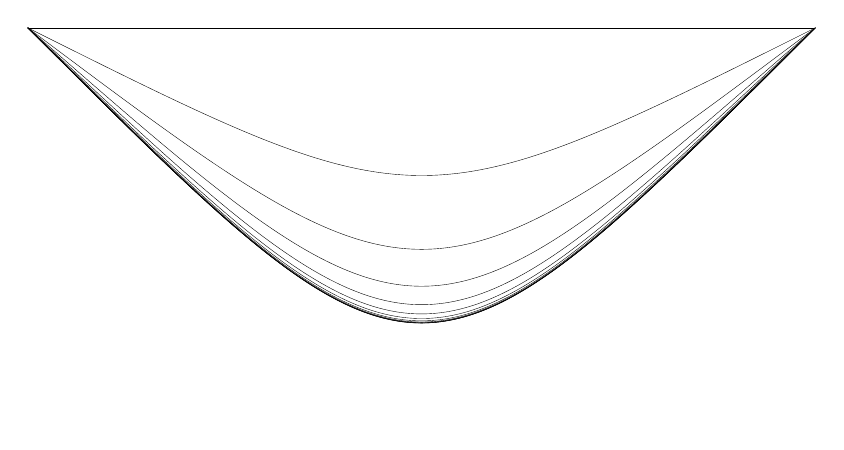
\begin{tikzpicture}[scale=5]
		\foreach \i in {0,1,2,...,12}{
			\draw[line width=0.05mm] (-1,1) .. controls (0,1/2^\i) .. (1,1);
		}
		\end{tikzpicture}
	\end{block}
	\vspace*{-1cm}
\end{frame}
\end{document}

\documentclass{amsart}
\usepackage[utf8]{inputenc}
\usepackage[english]{babel}
\usepackage{amsmath}
\usepackage{tikz-cd}

\newtheorem{theorem}{Theorem}
\newtheorem{lemma}[theorem]{Lemma}
\theoremstyle{definition}
\newtheorem{definition}[theorem]{Definition}

\newcommand{\N}{\mathbb{N}}
\newcommand{\Z}{\mathbb{Z}}
\newcommand{\R}{\mathbb{R}}
\newcommand{\HS}{\mathrm{HS}}
\newcommand{\dprime}{{\prime\prime}}
\DeclareMathOperator{\im}{im}
\DeclareMathOperator{\interior}{int}

\setlength{\textwidth}{\paperwidth}
\addtolength{\textwidth}{-1.4in}
\setlength{\textheight}{\paperheight}
\addtolength{\textheight}{-1.8in}
\calclayout

\newcommand{\p}{\mathrm{p}}
\newcommand{\q}{\mathrm{q}}

\begin{document}

\begin{definition}
	For $n \in \Z$ a continuous map is said to be \textit{$n$-homologically small} ---denoted $\HS_n$--- if the image of the map induced by $H_n(-)$ is finitely generated, and we say it is \textit{homologically small}, denoted $\HS$, if it is $\HS_n$ for every~$n$.
\end{definition}

\begin{definition}
	Let $X$ be a space and $f \colon X \to \R$ a function. For any $t \in \R$, the \textit{$t$-sublevel set of $f$} is defined by 
	\begin{equation*}
	X_{\leq t} = f^{-1}((-\infty, t]).
	\end{equation*}
\end{definition}

\begin{definition}
	Let $M$ be a metric space. For any $p \in M$ and $\epsilon \geq 0$ denote
	\begin{equation*}
	B_\epsilon(p) = \{q \in M\ |\ d(p,q) < \epsilon\}, \qquad
	\overline B_\epsilon(p) = \{q \in M\ |\ d(p,q) \leq \epsilon\}.
	\end{equation*}
\end{definition}

\begin{definition}
	Let $M$ be a metric space and $f \colon M \to \R$ a function.
	The space $M$ is said to be \textit{strongly locally-$f$-connected} if for each $p \in M$, $e > 0$, and $n \in \N$ there exists $\delta \in (0, e)$ such that for every $c \geq 0$ the image of the map induced by $H_n(-)$ on $B_\delta(p) \cap M_{\leq f(p)+\delta+c} \to B_e(p) \cap M_{\leq f(p)+e+c}$ is $0$.
\end{definition}

\begin{theorem} \label{t:strong local connectenss implies q-tameness}
	Let $M$ be a metric space and $f \colon M \to \R$ a function. If $M$ is strongly locally-$f$-connected and all level sets are compact, then, for any $s < t$ the inclusion $M_s \to M_t$ is $\HS$.
\end{theorem}

\begin{lemma} \label{l:commutative algebra}
	Given a commutative diagram of modules over a principal ideal domain
	\begin{equation*}
	\begin{tikzcd}
	A_{1,1} \arrow[r] & A_{1,2} & \\
	A_{2,1} \arrow[r] \arrow[u] & A_{2,2} \arrow[r] \arrow[u] & A_{2,3} \\
	& A_{3,2} \arrow[r] \arrow[u] & A_{3,3} \arrow[u]
	\end{tikzcd}
	\end{equation*}
	where the middle row is exact and both $A_{2,1} \to A_{1,1}$ and $A_{3,3} \to A_{2,3}$ have finitely generated images, then $A_{3,2} \to A_{1,2}$ does as well.
\end{lemma}

\begin{lemma} \label{l:neighborhood third}
	Let $M$ be a metric space. For any compact subset $K$ and open set $U$ with $K \subseteq U$ there exists a compact set $K^\prime$ such that
	\begin{equation*}
	K \subseteq \interior(K^\prime) \subseteq K^\prime \subseteq U.
	\end{equation*}
\end{lemma}

\begin{proof}
	For any $x \in K$ choose $\epsilon(x)$ such that $B_{\epsilon(x)}(x) \subseteq U$. We have
	\begin{equation*}
	B_{\frac{\epsilon(x)}{3}}(x) \subseteq \overline B_{\frac{\epsilon(x)}{2}}(x) \subseteq B_{\epsilon(x)}(x).
	\end{equation*}
	Since $K$ is compact, there exists a finite set $\{x_\lambda \in K\}_{\Lambda}$ such that $K \subseteq \bigcup_{\Lambda} B_{\frac{\epsilon(x_\lambda)}{3}}(x_\lambda)$. Defining $K^\prime = \bigcup_{\Lambda} \overline B_{\frac{\epsilon(x_\lambda)}{2}}(x_\lambda)$ finishes the proof.
\end{proof}

\begin{lemma} \label{l:key lemma for q-tameness}
	Let $M$ and $f$ be as in Theorem \ref{t:strong local connectenss implies q-tameness}.
	Consider sets $K, L \subseteq M$ with $K$ compact and $K \subseteq \interior(L)$. For any $s < t$ there is $\delta \in (0,\, t-s)$ such that $K \cap M_{s+\delta} \to L \cap M_{t}$ is $\HS$.
\end{lemma}

\begin{proof}
	The lemma holds for $\HS$ replaced by $\HS_{(n-1)}$ for any $n \leq 0$ since $H_{n-1}(-)$ induces the zero map. We will proceed by induction on $n$ assuming the lemma for $\HS_{(n-1)}$. 
	
	Given a compact set $L \subseteq M$ and $s < t$ let $\Sigma_{s, t}$ be the collection of all compact subsets $K$ of $\interior(L)$ for which there exists $\delta_K > 0$ and an open neighborhood $U_K$ of $K$ such that $U_K \cap M_{s+\delta_K} \to L \cap M_{t}$ is $\HS_n$.
	
	We start by showing that any point in $\interior(L) \cap M_s$ has a neighborhood in $\Sigma_{s, t}$.
	Let $x \in \interior(L) \cap M_{s}$ and take $e > 0$ such that $s + e < t$ and $B_e(x) \subseteq \interior(L)$.
	By the strong local-$f$-connectivity of $M$, there exists $\delta \in (0, e)$ such that for $c = s - f(x)$ the following composition is $\HS$:
	\begin{equation*}
	\overline B_{\delta/2}(x) \cap M_{s + \delta} \to
	B_\delta(x) \cap M_{s + \delta} =
	B_\delta(x) \cap M_{f(x) + c + \delta} \to
	B_e(x) \cap M_{f(x) + c + e} \to
	L \cap M_{t}.
	\end{equation*}  
	
	We will now show that the class $\Sigma_{s,t}$ is closed under finite unions.
	For $i \in \{1, 2\}$ let $K_i$ be in $\Sigma_{s,t}$ with $\delta_i > 0$ and $K_i \subseteq U_i$ open such that $U_{i} \cap M_{s+\delta_i} \to L \cap M_{t}$ is $\HS_n$.
	We Use Lemma \ref{l:neighborhood third} to construct sets $K_i^\prime$ such that
	\begin{equation*}
	K_i \subseteq \interior(K_i^\prime) \subseteq K_i^\prime \subseteq U_i.
	\end{equation*}
	Notice that for $\delta = \min(\delta_i)$ we have $K_i^\prime \cap M_{s+\delta} \to L \cap M_t$ is $\HS_n$.
	Additionally, the induction hypothesis implies that $K_1 \cap K_2 \cap M_s \to K_1^\prime \cap K_2^\prime \cap M_{s+\delta}$ is $\HS_{(n-1)}$.
	We therefore have the following commutative diagram satisfying the assumptions of Lemma~\ref{l:commutative algebra}:
	\begin{equation*}
	\begin{tikzcd}
	H_n(L \cap M_t) \oplus H_n(L \cap M_t) \arrow[r] &
	H_n(L \cap M_t) & \\
	H_{n}(K_1^\prime \cap M_{s+\delta}) \oplus H_n(K_2^\prime \cap M_{s+\delta}) \arrow[r] \arrow[u] & 
	H_{n}((K_1^\prime \cap M_{s+\delta}) \cup (K_2^\prime \cap M_{s+\delta})) \arrow[r] \arrow[u] &
	H_{n-1}(K_1^\prime \cap K_2^\prime \cap M_{s+\delta}) \\ & 
	H_{n}((K_1 \cup K_2) \cap M_s) \arrow[r] \arrow[u] &
	H_{n-1}(K_1 \cap K_2 \cap M_s). \arrow[u]
	\end{tikzcd}
	\end{equation*}
	We conclude that $K_1 \cup K_2 \in \Sigma_{s, t}$.
	Since any compact $K \subseteq \interior(L)$ can be expressed as a finite union of sets in $\Sigma_{s,t}$ the induction step and the lemma are proven.
\end{proof}

\begin{proof}[Proof of Theorem \ref{t:strong local connectenss implies q-tameness}]
	 It follows from applying Lemma~\ref{l:key lemma for q-tameness} to $K = M_{\leq s}$ and $L = M$.
\end{proof}

\end{document}

\section{Outlook}
%
\subsection{Two Alternative Conjectures}
In order to relate Morse's conditions to the above, we need a relative version of the $HLC^{\infty}$ condition.

\begin{defi}\label{defi:hlc}
Let $\mathcal{C}$ be a category with $0$ object and let $A\colon\mathbf{Top}\to\mathcal{C}$ be a functor. If $Y\subseteq X$ is a pair of topological spaces, we say that $Y$ is \emph{locally connected with respect to $A$ in $X$} if for each point $p\in Y$ and any open neighborhood $V$ of $p$ in $X$ there is an open neighborhood $U\subseteq V$ of $p$ such that $A(U\cap Y\hookrightarrow V)$ factors through 0.

We say that $Y$ is \emph{$HLC^{\infty}$ in $X$} if it is locally connected with respect to $\tilde{H}_*(-;\mathbb{Z})$ in $X$.
\end{defi}

We get the following rephrasing of strong local-$f$-connectedness.

\begin{prop}
Let $M$ be a metric space and $f\colon M\to\mathbb{R}$ a function. Then $M$ is strongly locally-$f$-connected if and only if $f_{\leq s}$ is $HLC^{\infty}$ in $f_{\leq t}$ whenever $s<t$.
\end{prop}
\begin{proof}
If each sublevel set is $HLC^{\infty}$ in larger sublevel sets, $M$ is clearly strongly locally-$f$-connected. For the converse direction, fix $s<t$ and choose some point $p\in f_{\leq s}$ with a neighborhood $V$ of $p$ in $f_{\leq t}$. We may choose $e\in(0, t-s)$ such that $B_e(p)\cap f_{\leq t}\subseteq V$. By strong local-$f$-connectedness, for each $d$ there is some $\delta\in(0,e)$ such that the map in reduced $d$-dimensional homology induced by $B_{\delta}(p)\cap f_{\leq s}\hookrightarrow B_e(p)\cap f_{\leq t}$ is trivial. The map $B_{\delta}(p)\cap f_{\leq s}\hookrightarrow V$ factors through the aforementioned map, so it is trivial in reduced homology, too. Thus, $f_{\leq s}$ is $HLC^{\infty}$ in $f_{\leq t}$.
\end{proof}

Note that the proposition gives a purely topological description of strong local-$f$-connectedness, so we can also use it to define strong local-$f$-connectedness for spaces that are not metrizable. It also yields the following corollary.

\begin{cor}
Let $M$ be a topological space and $f\colon M\to\mathbb{R}$ a function. If all sublevel sets are $HLC^{\infty}$, then $M$ is strongly locally-$f$-connected.
\end{cor}

We now propose the following generalization of \cref{prop:fin_dim_sing_hom}.

\begin{conj}\label{conj:q-tame_singular}
Let $Y\subseteq X$ be compact Hausdorff spaces such that $Y$ is $HLC^{\infty}$ in $X$. Then $\im H_d(Y\hookrightarrow X)$ is finite-dimensional for all $d$.
\end{conj}

As a persistent version, we have the following obvious consequence.

\begin{prop}\label{prop:q-tame_singular}
Let $M$ be a topological space and $f\colon M\to\mathbb{R}$ a function such that $M$ is strongly locally-$f$-connected, i.e., each sublevel set is $HLC^{\infty}$ in all larger sublevel sets. If \cref{conj:q-tame_singular} is true, then $H_{d}(f_{\leq\bullet})$ is q-tame for all $d$.
\end{prop}

In a similar spirit, we also propose the following conjecture as an analogue to \cref{cor:cech_sing_persistent_iso}.

\begin{conj}\label{con:d_I_0_sing_cech}
Let $M$ be a topological space and $f\colon M\to\mathbb{R}$ a function such that all sublevel sets are paracompact Hausdorff. If $M$ is strongly locally-$f$-connected, i.e., each sublevel set is $HLC^{\infty}$ in all larger sublevel sets, then 
\[
d_I(H_d(f_{\leq\bullet}),\CH_d(f_{\leq\bullet}))=0
\]
for all $d$.
\end{conj}

Here, $d_{I}$ denotes the interleaving distance between persistence modules. The conjecture is relevant because of the following criterion for q-tameness.

\begin{prop}
Let $M$ and $N$ be persistence modules such that $M$ is q-tame and assume $d_I(M,N)=0$. Then $N$ is q-tame.
\end{prop}
\begin{proof}
Pick indices $s<t$. Because $d_I(M,N)=0$, we may choose a $\delta$-interleaving with $\delta\in\left(0,\frac{t-s}{2}\right)$. Then we have a commutative diagram 

\[
\begin{tikzcd}
N_s\arrow[rrr]\arrow[rd]&&&N_{t}\\
&M_{s+\delta}\arrow[r]&M_{t-\delta}\arrow[ru]&
\end{tikzcd}
\]
so that the rank of $N_s\to N_t$ is bounded above by the rank of $M_{s+\delta}\to M_{t-\delta}$. The rank of $M_{s+\delta}\to M_{t-\delta}$ is finite by assumption, so $N$ is q-tame.
\end{proof}

Combining the previous result with \cref{prop:q-tame_singular}, we get the following.

\begin{cor}
If \cref{conj:q-tame_singular,con:d_I_0_sing_cech} are true, then so is \cref{con:q-tame_pers_cech_hom}.
\end{cor}

Thus, we have reduced our main conjecture to two smaller ones.

A possible proof strategy for \cref{conj:q-tame_singular} might be to adapt the proof strategy of Wilder's Finiteness Theorem, which is an analogue of \cref{prop:fin_dim_sing_hom} for sheaf cohomology, from \cite[Section II.17]{MR1481706}. Essentially the same proof also appears in \cite[Section III.10]{MR842190}.

A possible proof strategy for \cref{con:d_I_0_sing_cech} might be to adapt Bredon's proof of \cref{prop:cech_sing_hom_hlc} using his spectral sequence that relates \v{C}ech and singular homology.

\subsection{Q-Tameness of Persistent \v{C}ech Homology via Cosheaf Homology}\label{sec:cosheaf}
Note that what follows is rather informal and speculative.

When working with cohomology, the usual modern way to relate the singular and the \v{C}ech theory is via an intermediate step in the form of sheaf cohomology and then use the Leray and Grothendieck spectral sequences \cite[Chapter III]{MR1481706}. One might hope to use similar cosheaf theoretic methods, such as a possible theory of cosheaf homology, to obtain similar results for homology. So far, treatments of cosheaf homology are sparse. Among them are \cite{Andreotti.1973}, \cite{Schneiders.1987} and \cite{prasolov2018cosheaves}, but we are presently unable to determine whether the techniques in these texts can be adapted to our problems. Bredon, in \cite{Bredon.1968} and \cite[Chapter VI]{MR1481706}, also defines \v{C}ech homology with coefficients in a precosheaf and compares it to the singular theory for paracompact $HLC^{\infty}$-spaces \cite[Section VI.4 and Theorem VI.12.6]{MR1481706} using cosheaf theoretic methods. All of his results are still absolute comparison and finiteness results, i.e., they work for a single space $X$, so another obstacle, besides cosheaf homology being underdeveloped, is our desired generalization to subspaces $Y\subseteq X$ that are only $HLC^{\infty}$ in $X$ but not in themselves. That cosheaves might also help in overcoming this problem is suggested by the very nice formulation of the $HLC^{\infty}$ property in terms of precosheaves. The following definition appears in \cite{MR1481706}.

\begin{defi}
Let $\mathfrak{A}$ be a precosheaf on a space $X$ with values in a category with 0 object, i.e., a covariant functor on the poset category of open sets in $X$. We call $\mathfrak{A}$ \emph{locally trivial} if for all points $x\in X$ and all open neighborhoods $V$ of $x$ there is another open neighborhood $U\subseteq V$ of $x$ such that $\mathfrak{A}(U)\to\mathfrak{A}(V)$ factors through 0.
\end{defi}

The following definition is, up to our use of reduced homology, taken from \cite{Curry.2015}.

\begin{defi}
For any topological space $X$, we define the \emph{reduced Leray precosheaf} $\mathfrak{L}_X$ on $X$ as the precosheaf mapping $U\mapsto \tilde{H}_*(U;\mathbb{Z})$.
\end{defi}

\begin{defi}
If $f\colon Y\to X$ is a continuous map between topological spaces and $\mathfrak{A}$ is a precosheaf on $Y$, we define the \emph{pushforward of $\mathfrak{A}$ along $f$} as the precosheaf on $X$ mapping $U\mapsto\mathfrak{A}(f^{-1}(U))$. We denote it by $f_*\mathfrak{A}$.
\end{defi}

Now if $Y\subseteq X$ are topological spaces, we get an obvious morphism $i_*\mathfrak{L}_Y\to\mathfrak{L}_X$ of precosheaves on $X$, where $i\colon Y\hookrightarrow X$ is the inclusion, given by $\tilde{H}_*(U\cap Y\hookrightarrow U;\mathbb{Z})$. Note that the category of precosheaves with values in abelian groups is just a functor category from a small category to an abelian category. In particular, it has images given "pointwise". We get the following rephrasing of the relative $HLC^{\infty}$ property.

\begin{prop}
Let $Y\subseteq X$ be topological spaces. Then $Y$ is $HLC^{\infty}$ in $X$ if and only if $\im(i_*\mathfrak{L}_Y\to\mathfrak{L}_X)$ is locally trivial.
\end{prop}

Our hope is that one might be able to use this characterization in the future to prove the previously made conjectures.

\todo{Given $f\colon M\to\mathbb{R}$, is there a way of finding a single space (e.g. M itself, disjoint union of sublevel sets, colim of sublevel sets, hocolim of sublevel sets, continuously indexed mapping telescope (how to construct this?) of inclusions of sublevel sets, etc.) and a precosheaf with values in a category of persistence module (maybe the observable category) on that space such that $M$ is locally-$f$-connected iff that precosheaf is locally trivial?}

\section*{Acknowledgements}
This research has been supported by German Research Foundation (DFG) through the Collaborative Research Center SFB/TRR 109 \emph{Discretization in Geometry and Dynamics}, the Collaborative Research Center SFB/TRR 191 \emph{Symplectic Structures in Geometry, Algebra and Dynamics}, the Cluster of Excellence EXC-2181/1 \emph{STRUCTURES}, and the Research Training Group RTG 2229 \emph{Asymptotic Invariants and Limits of Groups and Spaces}.

\bibliographystyle{abbrvnaturl}
\bibliography{biblio}

\todos
\end{document}